\documentclass[11pt]{report}
% !TeX 

\usepackage[T2A]{fontenc}
\usepackage[utf8x]{inputenc}
\usepackage[english, russian]{babel}

\usepackage[T1]{fontenc}
\usepackage{titlesec, blindtext, color}
\usepackage[left=3cm, right=3cm, bottom=4cm, top=3cm, bindingoffset=0cm]{geometry}

\usepackage{amsmath}
\usepackage{mathtext}
\usepackage{environ}


\usepackage{wrapfig}
\usepackage{graphicx}
\usepackage{caption}
\usepackage{subcaption}
\usepackage{tabularx}


\graphicspath{{img/}}

\definecolor{gray75}{gray}{0.75}
\newcommand{\hsp}{\hspace{20pt}}
\addto\captionsrussian{\renewcommand{\contentsname}{Содержание}}

\titleformat{\chapter}[hang]{\Huge\bfseries}{\thechapter\hsp\textcolor{gray75}{|}\hsp}{0pt}{\Huge\bfseries}


\newenvironment{itemize*}%
  {\begin{itemize}%
    \setlength{\itemsep}{2pt}%
    \setlength{\parskip}{0.75pt}}%
  {\end{itemize}}


\newenvironment{enumerate*}%
  {\begin{enumerate}%
    \setlength{\itemsep}{2pt}%
    \setlength{\parskip}{0.75pt}}%
  {\end{enumerate}}

\newcolumntype{R}{>{\rule{0pt}{0.55cm}\raggedleft\arraybackslash}X}%
\newcolumntype{L}{>{\rule{0pt}{0.55cm}\raggedright\arraybackslash}X}%
\newcolumntype{C}{>{\rule{0pt}{0.55cm}\centering\arraybackslash}X}%
\newcolumntype{P}{>{\rule{0pt}{0.55cm}\centering\hsize=\dimexpr2\hsize+2\tabcolsep+\arrayrulewidth\relax}X}%

\newenvironment{wrapfigure*}%
 {%
  \setlength{\columnsep}{15pt}%
  \wrapfloat{figure}}%
 {\endwrapfloat}


\NewEnviron{myequation}{%
\begin{equation}
\scalebox{1.5}{$\BODY$}
\end{equation}
}



\title{
	\textbf{Escapy [ кодовое имя ]\\Дизайн документ}
}
\author{Генрих Тимур Домагальски}
\date{19.06.2017 Издаине 1}



\begin{document}
\maketitle



% Генерируем содержание
\tableofcontents


\newpage
\chapter*{Предисловие}
Данный документ не является окончательным со временем он будет дополняться новым материалом, так же претерпевать изменения как сугубо визуальные - с появлением изображений - так и концептуальные. Основная же задача документа состоит в том, что бы ознакомить читателя с общей идеей и стилистикой игры какой ее видит сам автор и в целом задать направление для дальнейшего процесса разработки. Автор, не являясь коренным носителем русского языка, заранее приносит свои извинения за возможные орфографические и лексические ошибки в тексте и просит относиться к ним с пониманием и снисходительностью.





\part{Вступление}
\chapter{Общие сведения}
Данный раздел содержит краткое описание концепции игры, ее историю, игровую механику, стилистику и прочее. Все из перечисленного будет подробнее описано в последующих главах. \newpage



\section{Концепция}
\paragraph{Игра} повествует о судьбе молодой девушки больной раком и потерявшей всю семью во время военного конфликта, а под конец своей короткой жизни вынужденной прибегать к наркотикам для усмирения боли и поддержания себя в физически функционирующем состоянии, чтобы отыскать девочку похищенную людьми предположительно убившими ее жениха. На протяжении всей игры гг будет идти по следам ее мертвого возлюбленного через всю юго-восточную Азию - постепенно узнавая новые подробности из его прошлой жизни она будет распутывать план грандиозной авантюры которую тот создал, вместе с тем болезнь главной героини будет стремительно развиваться, потребность в наркотиках возрастать, а преступный мир дичать.


\paragraph{Сюжетов} в игре два, при том точно сказать какой из них является основным довольно затруднительно, поэтому правильнее будет сказать что в игре на самом деле присутствует два главных персонажа и две линии повествования одна из которых постоянно пересекает другую, но только вместе они формируют картину в которой центральную идею занимает проблематика таких понятий как судьба, свобода, человечность и самое главное - жизнь с точки зрения философии экзистенциализма.

\section{Геймплей}
\paragraph{Жанр} представляет из себя кинематографический двухмерный платформер с относительно открытым миром в пределах сюжетной арки и боевой системой с некоторыми элементами метроидвании\footnote{\emph{https://www.wikiwand.com/en/Metroidvania}}, однако в остальных аспектах концептуально во многом от нее отличающийся.
\paragraph{Игровой процесс} напрямую связан с сюжетом игры - являясь, на ряду с окружающим игровым миром, неотъемлемым элементом повествования. В данном контексте аналогией, хоть и не вполне удачной может послужить литература эпохи романтизма в которой для подобных целей использовалась природа отражающая внутреннее состояние главного героя\footnote{\emph{http://manliness.ru/muzhskie-znaniya/osnovy-iskusstva-romantizm/}}. Другим примером могут послужить фильмы нуар из первой половины XX века, в них нередко характер и мотивы персонажей передаются с помощью расположения самих персонажей в кадре, а так же игры светотеней в их присутствии\footnote{\emph{http://kinoart.ru/archive/2013/04/formula-amerikanskogo-nuara}}. Возвращаясь к игровому процессу важно обратить внимание на то, что он не смотря свою особенно важную роль в формировании повествования не является ключевым аспектом игры, но составляет часть общего депрессивного сеттинга\footnote{\emph{https://www.wikiwand.com/en/Setting\_(narrative)}} - переполненного фатализмом\footnote{\emph{https://www.wikiwand.com/en/Fatalism}}, насилием и безысходностью преступного мира всячески не принимающего главную героиню и вместе с тем не желающего ее отпускать.

\paragraph{Игровая механика} в первую очередь завязана на борьбе с болью которую постоянно испытывает больная раком главная героиня. Способов борьбы с ней несколько, однако самым основным и проверенным являются наркотики которых в игре полное множество. От уровня боли сильно зависят физические способности героини, кол-во получаемого ею урона, возможность использовать специальные умения, а так же психическое состояние ГГ и что за этим следует - восприятие окружающего мира.
\paragraph{Смерть} в игре отсутствует, вместо этого ГГ теряет сознание тем самым отправляется в мир ласковых грез и воспоминаний, который между тем подвержен де конструкции и фрагментации. По мере развития сюжета, а в месте с ним болезни и физической и психической деградации героини, мир грез будет постепенно рассыпаться превращаясь в подобие кошмарного лабиринта воспаленного сознания. Хорошей метафорой здесь послужит кусочек бумаги брошенный в костер - временами можно заметить, как под жаром огня, тлеющий кусочек бумаги уносится в воздух медленно и красиво рассыпаясь. Так же стоит отметить, что фактическое отсутствие возможности умереть с одной стороны подчеркивает фаталистический характер сюжета, с другой переносит повествование в более кинематографическую плоскость позволяя игроку в большей степени сосредоточится на сюжете и сеттинге, не теряя вместе с тем динамизма присущего играм.
\paragraph{Потеря сознания} в зависимости от контекста может длиться несколько секунд не неся в себе какой либо сюжетной нагрузки или же наоборот - самой являться частью сюжета, раскрывая с одной стороны прошлое персонажа, а с другой ее актуальное психическое состояние, мысли, страхи и переживания - что в идеале должно позволить создать сильную эмоциональную связь между игроком и главным героем. Данный факт делает этот элемент игровой механики одним из самых важных в формировании нарратива.
\paragraph{Наркотики} являются основным способом борьбы с болью. В игре присутствует много разных видов наркотиков, у каждого из них свои особенности, побочные отрицательные и положительные эффекты, степени привыкания и чистоты. Наркотики можно подбирать, покупать или создавать самому.
\paragraph{Мертвый жених} является настоящим главным героем игры, он создал и запустил в действие план нацеленный на прекращение нелегальной торговли детьми, однако в определенный момент что то пошло не так и он погиб. Главная героиня начав расследовать его прошлое что бы найти зацепки в поисках пропавшей девочки постепенно начинает узнавать подробности и все больше погружаясь в мир криминала движется к истокам. 


\section{Место действия и окружение} 
\paragraph{Сюжет} развивается на просторах целого мира, однако подавляющая часть действия происходит в регионе восточной и юго-восточной Азии. Характерной особенностью данного региона является сильно выраженный культурный контраст, чрезвычайно высокая плотность населения и значительный разрыв уровня жизни в зависимости от страны.\footnote{\emph{https://www.wikiwand.com/en/East\_Asia}} \footnote{\emph{https://www.wikiwand.com/en/Southeast\_Asia}} Сюжет поделен на логически и хронологически связанные арки, каждая из которых как правило развивается на территории какой то одной из стран региона. Повествование начинается в восточной Европе в стране пост-советского пространства с короткой истории из детства главного персонажа, затем ненадолго переносится в западную Европу где происходит завязка сюжета, однако основное действие начинается после прибытия главного персонажа в богатую и спокойную Японию в Токио, а заканчивается в Таиланде в Бангкоке - городе нищеты, проституции, наркотиков и безвкусно обставленных баров.
\paragraph{Сеттинг} мрачный мир криминала юго-восточной Азии, полный социального неравенства и неоправданного ультра насилия. Доминирующая цветовая гамма - вечерняя, отражающая внутреннее состояние главного персонажа. По мере развития сюжета гамма постепенно изменяется от яркого вечернего неба, до темной ночи, тем самым натуральные краски засыпающей меланхоличной природы сменяются контрастными огнями полных жизни, никогда не спящих ночных городов. Окружение игрового мира переполнено деталями главная цель которых состоит в том, что бы усилить эффект погружения в происходящее.\footnote{\emph{https://cutinsight.com/samyj-yarkij-slow-motion-v-filmah-tarantino/}} \footnote{\emph{https://www.youtube.com/watch?v=GLy8HcCI4qU}} \footnote{\emph{https://goo.gl/HPiogi}}
Особое внимание так же уделено богатой детализированной анимации, без которой не возможно создать ощущение живости персонажей и тем самым создать с ними сильную эмоциональную связь.


\section{Особенности}
\paragraph{Главной особенностью} игры является ее направленность в первую очередь на создание глубокой истории вызывающей сильную эмоциональную реакцию. Геймплей  выступает лишь в роли инструмента повествования, так же как это делает камера в кинематографе, а  
игра в данном случае превращается в артхаус\footnote{\emph{https://www.wikiwand.com/en/Art\_film}} из мира игр, будучи переполненной смыслами в которой абсолютно все из окружения имеет свое строгое предназначение - будь то аллюзия на работы Сартра\footnote{\emph{http://taby27.ru/sdachi-rabot/sdacha\_rabot\_po\_folosofii/706.html}} или же банальная экспрессия, но в конечном итоге оставляет за игроком полную свободу интерпретации. 

В свою очередь для достижения упомянутого уже много раз эффекта кинематографичности игра прибегает к некоторым хитрым приемам, как например:\begin{itemize*}
\item Ограничение количества кадров изображения в секунду до 25.
\item Каширование\footnote{\emph{https://goo.gl/tmp7ow}} экрана в особо динамичных моментах игры.
\item Активное применение пост-обработки под которую заточен движок игры.
\item Необычная для двухмерной игры боевая система, которой посвещена отдельная глава документа.\\
\end{itemize*}


\section{Целевая аудитория}
Предполагается, что игра способна заинтересовать часть аудитории 16+. Стоит учесть что присутствие в игре ультра-насилия и наркотиков как элемента механики может в некоторых странах создать определенные проблемы с лицензированием даже для категории 18+. \\ 


\section{Предпосылки и источники вдохновения}
Концептуально игра не имеет аналогов в своем жанре или автор о таких не знает, единственным исключением может стать <<\textit{The last night}\footnote{\emph{http://store.steampowered.com/app/612400/The\_Last\_Night}}>>, о котором на данный момент мало что известно сверх того, что разработка над ним ведется несколько лет.

В плане геймплея игра использует некоторые удачные решения из других не только двухмерных игр, в первую очередь речь идет о: \begin{itemize*}
\item Играх в жанре JRPG\footnote{\emph{https://goo.gl/TBoCEs}} и Metroidvania откуда был заимствован открытый мир, хорошим примером может послужить <<\textit{Child of light}>>
\item <<\textit{Bioshock burial at sea}>> - тут нужно сразу заметить, что речь идет в первую очередь о мотивации главной героини, сюжетных приемах использованных в игре, а так же эмоциональной окраске сюжета и сеттинга.
\end{itemize*} Помимо игр к категории очевидных источников вдохновения можно отнести такие примеры из кинематографа и анимации как: \begin{itemize*}
\item <<\textit{Реквием по мечте}>> и <<\textit{Черный лебедь}>>
\item <<\textit{Только бог простит}>> и в целом большинство фильмов Николаса Виндинга Рефна
\item <<\textit{Пираты черной лагуны}>> и <<\textit{Ковбой бибоп}>>\\
\end{itemize*}


\section{Платформы}
На данный момент только PC.

\section{Мультиплеер}
Не предпологается.

\part{Концепция}


\chapter{Сюжет}
Сразу следует отметить, что в этой главе рассматривается не сам сюжет, а его концептуальная состовляющая как например ведущая проблематика, мотивация и форма. Для ознакомления с самим сюжетом стоит обратиться к отдельному документу.

Автор данной версии издания документа скромно просит еще раз обратить внимание на тот факт, что он не является коренным носителем русского языка, а так же на то, что философ модернист он только в душе, в то время как основой род его деятельности имеет технический характер.


\newpage
\section{Форма}
Сюжет имеет нелинейный характер повествования и складывается из двух отдельных, но пересекающихся между собой ветвей истории главных персонажей. При этом один из них на момент начала игры уже де-факто мертв и его историческую линию игрок может наблюдать только глазами второго главного героя - девушки и только в обратном хронологическом порядке. Полная картина происходящего формируется как мозаика из пазлов ближе к концу третей арки (3/4 продолжительности игры и сюжета) и станет кульминацией истории, хотя наиболее динамичная и эмоциональная часть в игре - последняя.

Сам по себе сюжет имеет изменчивую скорость - депрессивная и меланхоличная в начале и ураганная под конец, что находит свое отображение в геймплее.

\section{Мотив}
Фоном для основной проблематики и ведущим движителем сюжета является история бывшего гангстера - ныне мертвого возлюбленного главной героини, которая в попытке разобраться в случившемся оказывается втянутой в опасную авантюру спланированую покойным чтобы перекрыть выросший до безумных размеров поток работарговли - в первую очередь женщинами и детьми\footnote{\emph{http://repin.info/kriminalnoe-chtivo/kitay-dikosti-sovremennoy-rabotorgovli}}, которым заправляют несколько самых опасных преступных группировок азии (триад)\footnote{\emph{https://www.wikiwand.com/en/Triad\_(organized\_crime)}} \footnote{\emph{http://atimemag.ru/details/triads/}}. Героиня потеряв все в жизни второй раз подряд и узнав в добавок что больна раком находит смысл жизни в спасении пропавшей девочки по совместительству <<дальней родственницы>> покойного, а на самом деле жертвы работарговцев. 


\section{Проблематика}
Ключевой темой и идеей игры, является, как было уже сказано в начале документа, проблематика фундаментальных понятий экзистенциализма - где начинается и заканчивается человечность, существует ли судьба и что из себя представляет настоящая свобода? К вышеперечисленному в конечном итоге сводятся все аспекты игры, будь то на уровне символизма - аккуратными и не очень намеками со стороны самого сюжета и геймплея, как например работорговля, смертельная болезнь и наркозависимость, так и со стороны самого повествования - сюжетной линии главной героини - ее поступков, выборов и мотивов. Лично автор когда говоря об экзистенциализме - понимает его согласно Сартровской трактовке и в первую очередь это касается понятия свободы, которая согласно Сартру является абсолютной и уже из нее рождается все остальное - человек имеет свободу выбора независимо от условий, даже будучи заключенным он в конечном итоге может быть свободнее свое сторожа. Именно эта концепция пронизывает всю сюжетную линию и сущность главной героини, которая является вечным заложником трагических обстоятельств.


\section{Деление сюжета на части - <<арки>>}
Повествование поделено на четыре связанные между собой хронологически  и логически части, каждая из которых имеет свою уникальную стилистику, настроение и динамику повествования - иными словами сюжетный мотив. Ниже представлен список арок в их хронологическом порядке:
\begin{enumerate}
\item <<\textit{Лимб}>> - Полная рутины, но все же счастливая жизнь обрывается кошмарным образом, жених погибает, ребенок исчезает, а у гг обнаруживается рак. Жизнь теряет смысл.
\item <<\textit{Нить}>> - Цель найти ребенка становится единственным смыслом жизни, за который гг хватается всеми силами, осознавая что таким выбором она \textit{де-факто} подписывает себе смертный приговор.
\item <<\textit{Наследие}>> - Кульминация сюжета, история гг и ее покойного жениха собирается в целостную картину, ребенка в свою очередь спасти не удается.
\item <<\textit{Освобождение}>> Смерть главной героини.
\end{enumerate}
Названия частей не являются случайными - они отражают доминирующую в данный момент повествования идею, однако чтобы понастоящему понять данные названия следует ознакомится с полноценным сюжетом, которому не местом в концептуальном документе.


\chapter{Сеттинг}
Глава содержит более подробное описание местности на которой происходит развите сюжета - ее харрактеристические черты, историю уникальную атмосферу и тп.

\newpage
\section{Югославия}

Участие данного реигона как в сюжете так и в самой игре минимально, однако его стоит упомянуть так как югославия является родиной главной героини, раннее детсво которой пришлось на военные конфликты в этой стране перед ее окончательным развалом. В этих военных конфликтах погибла вся семья ГГ. В игре действие в югославию переносится очень редко и на коротки промежуток времени -  как правило в виде отрывков воспоминаний и редких снов. Исключением является очень короткое начало игры которое происходит в косове\footnote{\emph{https://goo.gl/TZPuUT}} - игрок при этом не видит непосредственно гибели семьи, вместо этого ему показываются разрушения и вооруженные люди которые не обращают внимания на ребенка.

\vspace{8ex}
\begin{center}
	\begin{figure}[h]
		\begin{subfigure}{.5\linewidth}
			\includegraphics[width=\linewidth]{img/eps/balkan}
  			\caption{Бывшая Югославия.}
  			\label{img:balkans}
		\end{subfigure}
		\hfill
		\begin{subfigure}{.5\linewidth}
			\includegraphics[width=\linewidth]{img/eps/kosovo}
  			\caption{Косовская война.}
  			\label{img:kosovar}
		\end{subfigure}
	\end{figure}
\end{center}



\newpage
\section{Сумрачный Лондон}

В Лондоне начинается основной сюжет и развивается на протяжении целой арки, здесь главная героиня знакомится с главным героем из Азии и его <<\textit{двоюродной сестрой}>> которую он с собой привез. Не смотря на то, что арка сама по себе короткая ее значимость очень велика, тк именно здесь происходит завязка сюжета - жениха убивают, девочка исчезает, квартира сгорает, а у героини диагностируют лейкоз. Здесь главная героиня встречает экзистенциальный кризис, теряет смысл жизни, а потом находит новый. Так депрессивный и меланхоличный мотив отражается на окружающем мире, потому Лондон в 
\setlength{\intextsep}{2pt}
\setlength{\columnsep}{10pt}
\begin{wrapfigure*}{l}{0.7\linewidth}
	\centering
	\begin{center}
		\includegraphics[width=.95\linewidth]{img/eps/l5}
	\end{center}
\end{wrapfigure*} игре изображен в серо-голубых тонах с очень низким контрастом окружения и плохой еле-дождливой погодой и вечернем времени суток. В светлых и теплых тонах Лондон будет появляться только в воспоминаниях главной героини о прошлом времени проведенном вместе со своим женихом и его маленькой родственницей во время потери сознания и просто обыкновенных флешбеков.

\clearpage
\begin{center}
	\begin{figure}[h]
		\centering
		\begin{center}
			\includegraphics[width=.96\linewidth]{img/eps/l2}
		\end{center}
		\vfill
		\vspace{0.3cm}
		\begin{center}
			\includegraphics[width=.96\linewidth]{img/eps/l1}
		\end{center}
	\end{figure}
\end{center}


\clearpage
\section{Юго-восточная и восточная азия}
\begin{figure}[!b]
	\begin{center}
		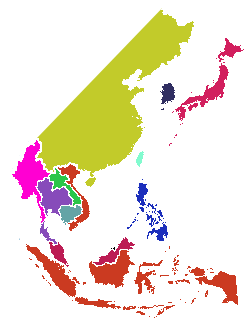
\includegraphics[width=.7\linewidth]{img/eps/asi_web_2}
  		\caption{Юго-восточная азия.}
  		\label{img:asia}
	\end{center}
\end{figure}
Этот регион без сомнений можно назвать самым важным в игре, поскольку здесь происходит 90\% сюжета. Отличительной чертой юго-восточной Азии является чрезвычайно высокий уровень плотности населения, высокий уровень контраста в культуре и качестве жизни между странами - в первую очередь между южной и восточной частями региона.

Основной сюжет начинается после приезда главной героини в Японию, затем в каждой из сюжетных арок действие переносится в другие страны - как правило каждая следующая арка проходит в стране большим уровнем бедности и преступности чем в предыдущей. Заканчивается сюжет в Таиланде в Бангкоке.

\clearpage
\subsection{Япония, Токио}
\paragraph{Япония} - Третья по уровню ВВП страна в мире, первая по уровню покупательской способности и безопасности жизни. Преступный мир в принципе отсутствует, якудза кражами и убийствами не занимается, а только контролирует публичные дома и мелкий игорный бизнес. Наркотиков мало, добыть сложно, а если то за высокую цену. Однако во второй арке, которая происходит в Японии, наркотики главной героине почти не нужны. 

Застройка как правило невысокая, улицы чистые, все провода выведены наружу. Доминирующая гамма в игре - начало заката - оранжевые и светло-фиолетовые тона.

\vspace{8ex}
\begin{center}
	\begin{figure}[h]
		\begin{subfigure}{.5\linewidth}
			\includegraphics[width=.97\linewidth]{img/eps/t1}
		\end{subfigure}
		\hfill
		\begin{subfigure}{.5\linewidth}
			\includegraphics[width=.97\linewidth]{img/eps/t2}
		\end{subfigure}
		\vfill
		\vspace{2ex}
		\begin{subfigure}{.5\linewidth}
			\includegraphics[width=.97\linewidth]{img/eps/t4}
		\end{subfigure}
		\hfill
		\begin{subfigure}{.5\linewidth}
			\includegraphics[width=.97\linewidth]{img/eps/t5}
		\end{subfigure}
	\end{figure}
\end{center}

\clearpage
\subsection{Южная корея, Сеул}
В целом может показаться что Ю.К. эстетически во много похоже на Японию. Ее отличительной особенностью от последней в первую очередь является население - которое в большинстве своем католическое. Поэтому не смотря на схожесть застройки, которая в прочем в Корее более высокая чем в Японии, на улицах можно спокойно встретить католические храмы с неоновыми распятиями.
У Корее нет собственной сюжетной арки, ее она делит с Японией как и цветовую гамму.

\vspace{8ex}
\begin{center}
	\begin{figure}[h]
		\begin{subfigure}{.5\linewidth}
			\includegraphics[width=.97\linewidth]{img/eps/se1}
		\end{subfigure}
		\hfill
		\begin{subfigure}{.5\linewidth}
			\includegraphics[width=.97\linewidth]{img/eps/se2}
		\end{subfigure}
	\end{figure}
\end{center}

\newpage
\subsection{Просто Гонконг}
Просто столица преступного мира Азии. Вечно окутанные то ли туманом, то ли смогом - никогда не засыпающие бетонные джунгли стали домом для более чем пятидесяти\footnote{\emph{https://www.wikiwand.com/en/Triad\_(organized\_crime)}} самых жестоких и влиятельных преступных группировок Азии и всего мира в их числе:
\setlength{\columnsep}{5pt}
\begin{wrapfigure*}[5]{r}{0.7\linewidth}
	\centering
	\begin{center}
		\includegraphics[width=\linewidth]{img/eps/k9}
	\end{center}
\end{wrapfigure*}
\begin{itemize}
\item 14K
\item Sun Yee On
\item Tai Huen Chai
\item Wo Shing Wo
\item Shui Fong
\item Wo Hop To
\item Luen Group
\\ \\ \\ \\
\end{itemize}
К сведению одна лишь триада 14К насчитывает порядка двадцати пяти тысяч членов и принимает участие всех возможных видах нелегального бизнеса Азии и считается самой сильной преступной группировкой в мире. 
\begin{center}
	\begin{figure}[h]
		\begin{subfigure}{.82\linewidth}
			\includegraphics[width=1\linewidth]{img/eps/k3}
		\end{subfigure}
	\end{figure}
\end{center}

\begin{figure}
	\centering
	\includegraphics[height=1\textheight]{img/eps/k1}
\end{figure}

\subsection{Вьетнам, Ханой}
Столица Вьетнама, очень грязно, очень людно и очень много мопедов, а еще через этот город идет трафик нелегальных товаров - как например похищенные люди или опиум выращенный где то в Лаосе, Таиланде или том же Вьетнаме. Собственной вменяемой мафии как таковой нет, в целом бедно но спокойно - в игре это остановка на пути в Таиланд.\\
\begin{center}
	\begin{figure}[h]
		\begin{subfigure}{.77\linewidth}
			\includegraphics[width=.99\linewidth]{img/eps/hanoi}
		\end{subfigure}
	\end{figure}
\end{center}		
\begin{center}
	\begin{figure}[h]
		\begin{subfigure}{.77\linewidth}
			\includegraphics[width=.99\linewidth]{img/eps/hanoi2}
		\end{subfigure}
	\end{figure}
\end{center}	

\clearpage
\subsection{Тайланд, Бангкок}
Страна слонов, секс-туризма, наркотиков, проституции, работарговли \footnote{\emph{https://www.kommersant.ru/doc/2759684}}, плохо оформленных баров, тайского бокса и трущоб граничащих с небоскребами. Именно сюда в конечном итоге приводят все ниточки истории.
\setlength{\intextsep}{.5pt}
\begin{center}
	\begin{figure}[h]
		\begin{subfigure}{.94\linewidth}
			\includegraphics[width=1\linewidth]{img/eps/th1}
		\end{subfigure}
	\end{figure}
\end{center}	
\begin{center}
	\begin{figure}[h]
		\begin{subfigure}{.94\linewidth}
			\includegraphics[width=1\linewidth]{img/eps/th2}
		\end{subfigure}
	\end{figure}
\end{center}	



\chapter{Музыка и звуки}
Эта очень коротка глава представляет из себя скорее сборник ссылок на творчество разных музыкальных исполнителей и групп, которые как автор считает по своему духу или форме в большей или меньшей степени передают настроение, атмосферу или идею всей игры, или же некоторых ее эпизодов - возможно даже очень коротки, но от того не менее значимых. Разумеется о вкусах не спорят, а автор не претендует на звание знатока или эксперта и поэтому не исключено что даже не догадывается о существовании произведений которые могут
передавать сеттинг игры гораздо лучше чем произведения из списка автора. Именно поэтому дополнение этой главы новым контентом особенно приветствуется.
\newpage

\section{Ссылки на музыкальные произведения}

\textit{Moderat - Damage Done}\footnote{\emph{https://www.youtube.com/watch?v=8a6U8XbTx0I}}
\\
\textit{Moderat - Let in the Light}\footnote{\emph{https://www.youtube.com/watch?v=eD6MeGYG7Ok}}
\\
\textit{Cigarettes After Sex - Affection}\footnote{\emph{https://www.youtube.com/watch?v=5soixb2U6xM}}
\\
\textit{Julian Winding - The Demon Dance}\footnote{\emph{https://www.youtube.com/watch?v=OvUJsu5w8IU}}
\\
\textit{Burial - Untrue}\footnote{\emph{https://www.youtube.com/watch?v=X-VmiLA3nqg}}
 

\chapter{Персонажи}
В данной главе содержится более подробное описание игровых персонажей - их история, характер, внешний вид и т.п. Автор выражает, что в процессе разработки данная глава будет разрастаться новым контентом - в первую очередь графическим, а так же,  что к моменту выхода второго издания история главных персонажей будет отшлифована и переписана в более структурированном виде, а раздел сюжетных персонажей обзаведется несколькими новыми личностями.

\newpage
\section{Главные персонажи}

\subsection{Главная героиня}
\setlength{\columnsep}{15pt}
\setlength{\intextsep}{2pt}
\begin{wrapfigure*}{r}{0.44\textwidth}
\centering
	\begin{center}
		\begin{tabularx}{.44\textwidth}{ |L|L| }
  			\hline
  			\multicolumn{2}{|P|}{Bio} \\
  			\hline
  			Категория & ГГ \\
  			\hline
  			Имя & <<.?.>> \\
  			\hline 
  			Пол & Женский \\
  			\hline
			Возраст & 23 года \\
  			\hline
  			Национальность & Балканы \\
  			\hline
		\end{tabularx}
	\end{center}
	\includegraphics[width=1\linewidth]{img/eps/yugoslav}
  	\caption{Милое детство.}
  	\label{img:yugoslav}
\end{wrapfigure*} 
Молодая девушка, 23 года, точная дата и место рождения неизвестны. Предположительно балканского происхождения. На период ее раннего детства пришлась череда югославских войн в которой она потеряла всю семью, от голодной и холодной смерти спаслась по счастливой случайности благодаря тому что ее заметил миротворцев. В лагере для беженцев вместе с другими детьми с похожей судьбой была вывезена религиозной благотворительной организацией в Италию где до совершеннолетия жила в монастырском приюте для сирот. Взросление внутри религиозного института, наряду с потерей всей семьи лишь подкрепило ее уверенность в отсутствии бога, сформировав циничный взгляд на мир и уверенность только в своих собственные способностях. В целом до событий игры обладала весьма скверным характером, что можно понять, однако ей повезло не помнить пережитых ужасов войны и потому сформироваться как полноценной личности и лишь изредка мучиться от непонятных снов о детстве. Покинув приют поступила во флорентийский университет, а после получения диплома по экономии перебралась в Великобританию, где получила должность в одной из контор в Лондон-сити и познакомилась со своим женихом американояпонского происхождения. К моменту начала событий игры прожила 2 года вместе с ним и его восьмилетней двоюродной сестрой, однако дальнейшую счастливую жизнь прервало убийство возлюбленного на ее глазах и две пули в легком. Придя в сознание в больнице гг узнает что у нее прогрессирующий лейкоз на второй стадии, ребенок пропал, квартира сгорела, а в голове то и дело вертится сцена убийства, при этом все действия полиции не приносят каких либо результатов поскольку преступники оказались быть членами иностранной ОПГ и покинули страну еще в тот же самый день. Потеряв все, в том числе и смысл жизни, гг в конце концов находит последний в спасении девочки, однако единственной зацепкой в ее поисках оказывается личность покойного жениха, прошлое которого ведет примяком в японию.

Попав в Японию она медленно погружается в криминальный мир и ступая по следам своего покойного мужа путешествует через всю юго-восточную Азию. Будучи довольно хрупкой и не приспособленной к тяжелым физическим нагрузкам добавив к этому прогрессирующий рак, даже приняв наркотик или стимуляторы ее нельзя назвать профессиональным бойцом, так что абсолютно все вооруженные стычки с бандитами можно охарактеризовать только одним словом - выживание.\\

\subsection{<<?>> Мертвый жених}
\setlength{\columnsep}{15pt}
\setlength{\intextsep}{2pt}
\begin{wrapfigure*}{r}{0.44\textwidth}
\centering
	\begin{center}
		\begin{tabularx}{.44\textwidth}{ |L|L| }
  			\hline
  			\multicolumn{2}{|P|}{Bio} \\
  			\hline
  			Категория & ГГ \\
  			\hline
  			Имя & <<.?.>> \\
  			\hline 
  			Пол & Мужской \\
  			\hline
			Возраст & 30 лет \\
  			\hline
  			Национальность & Америка/Япония \\
  			\hline
		\end{tabularx}
	\end{center}
	\includegraphics[width=1\linewidth]{img/eps/hanoi}
  	\caption{Типичный Ханой.}
  	\label{img:hanoi}
\end{wrapfigure*} 
Отец американец, мать японка, таких в японии называют <<\textit{хафу\footnote{\emph{https://goo.gl/MHztAw}}}>>, с виду больше похож на американца - ростом выше, кожа светлее. Детство пришлось на период потерянного десятилетия, поэтому рост пришлось в условиях благородной бедности, как впрочем большинству населения Японии тогда. Мать погибла в автокатастрофе когда ему было 14, а спустя 5 лет в таких же условиях погиб отец. Семьи со стороны отца у него не было, а пожилые консервативные родственники матери отказались помогать сыну <<шлюхи переспавшей с гайдзином>> поэтому пришлось бросать вуз и идти работать. Однажды желая поднять немного прибыли сверху он устроился охранником в нелегальном игровом зале, там по счастливой случайности оказалось что якудзе нужны люди с хорошим знанием английского, а он говорит на английском как на родном - так и началось его движение по теневой карьерной лестнице. Его новая работа зачастую заключалась лишь в переговорах с иностранцами без необходимости проливать чью либо кровь. За 3 года до событий игры, герой на несколько дней отправляется на очередную рутинную встречу в Ханой, где случайно попадает на встречу торговцев детьми из Китая и Таиланда, которых официально не существует\footnote{\emph{https://goo.gl/rzDcTs}} либо просто похитили. Там он спасает девочку, а по возвращению в Японию у него появляется план как прикрыть этот бизнес. В течении следующего года он прорабатывает и подготавливает план, началом которого служит его поездка в Европу, однако в определенный момент что то идет не так и его убивают. 

\newpage
\section{Сюжетные персонажи}
\subsection*{Важная заметка}
Данная секция должна пополняться по мере появления детального сюжета.

\subsection{Похищенная девочка}
\setlength{\columnsep}{15pt}
\setlength{\intextsep}{2pt}
\begin{wrapfigure*}{r}{0.44\textwidth}
\centering
	\begin{center}
		\begin{tabularx}{.44\textwidth}{ |L|L| }
  			\hline
  			\multicolumn{2}{|P|}{Bio} \\
  			\hline
  			Категория & Сюжет \\
  			\hline
  			Имя & <<.?.>> \\
  			\hline 
  			Пол & Женский \\
  			\hline
			Возраст & 8 лет \\
  			\hline
  			Национальность & <<?>> \\
  			\hline
		\end{tabularx}
	\end{center}
\end{wrapfigure*} 
О прошлом почти ничего не известно, предположительно родилась в Китае в бедной многодетной семье и в возрасте 5 лет была ею продана.\footnote{\emph{http://repin.info/kriminalnoe-chtivo/kitay-dikosti-sovremennoy-rabotorgovli}} Была замечена <<?>> главным персонажем в Ханой и выкуплена, в последствии жила с ним в Японии как дальняя родственница так как внешне от типичной японки не отличалась. Внешность типичная азиатская - черные и густые волосы, темные глаза и рост немного меньше чем у западных ровесников. После убийства <<?>> главного персонажа исчезла, но что именно с ней произошло неизвестно.

\chapter{<<NPC>>}
Это глава полностью посвящена игровым персонажам не обладающим какой либо сюжетной ценностью, однако являющимися частью игровой механики и повествования. В данной версии издания она фактически пустует, но со временем будет пополняться новым контентом. 


\section{Нейтральные}
\section{Враждебные}


\part{Функциональные аспекты игры}
\chapter{Геймплей}
Данный раздел содержит более глубокое описание игрового процесса и всего что его касается в первую очередь с технической стороны вопроса.

Отдельно стоит заметить, что в данной главе не редко появляются математические формулы вычислений значений разных игровых параметров. Читатель может иногда заметить нотацию вида:
\begin{myequation}
		variable_{<a,b>} = ...
\end{myequation}
Что в принципе является просто удобной записью сокращением, при которой сразу подан диапазон допустимых значений переменной, иным способом это можно записать как: 
\begin{myequation}
		variable \in [a,b]
\end{myequation}
В случае если при записи переменной данная нотация не использовалась значит эта переменная имеет единичный диапазон допустимых значений, что можно записать как: 
\begin{myequation}
		variable \in [-1,1]
\end{myequation}
Математиков автор просит закрыть глаза.
\newpage

\section{Передвижение по миру}
\subsection{Характеристика внутриигрового мира}
Игра предусматривает наличие открытого для изучения и передвижения мира и дает игроку свободу перемещения по нему в пределах сюжетной арки. Сюжетная арка включает в себя одну или несколько мегалокаций стилистических связанных между собой. Арки отличаются между собой характером и стилистикой, однако внутри являются стилистически замкнутыми и полными.
Иными словами общий мир игры является совокупностью мегалокаций между которыми движение возможно только через сюжетную линию, в свою очередь мегалокации являются совокупностью локаций поменьше - между которыми движение уже полностью открыто для игрока. Каждая арка обладает своей собственной стилистикой, которая однако является доминирующей внутри самой арки.

\subsection{Список основных локаций}
Игровой мир предствален следущими мегалокациями (Список в хронологическом сюжетном порядке): \begin{enumerate*}
\item Лондон
\item Токио и Сеул
\item Гонконг
\item Ханой и Бангкок
\end{enumerate*}

\section{Взаимодействие с окружением}
Взаимодействие с окружением это очень важный элемент повествования и геймплейя. Переполненное деталями окружение дает игроку полную свободу для своего изучения или модификации. Большинство объектов окружения имеют ту или иную физическую интерпретацию позволяя на физическое взаимодействие с собой - например кружку на столе можно с него с бросить или например подобрать лежащий на земле предмет и его использовать или добавить в свой инвентарь. 

Так же важной частью окружения являются несюжетные и неигровые персонажи <<NPC>> - некоторые из них могут быть нейтрально ил настроены по отношению к игрок, другие же наоборот враждебно. С некоторыми из них можно взаимодействовать например с помощью диалогов или же вступить в бой. Поведение и стилистическое выполнение таких персонажей зависит в первую очередь от данной игровой локации.
\subsection{Список некоторых видов взаимодействий}
Следует заметить что не все из ниже перечисленных возможностей могут быть доступны в полном объеме, как правило для разных предметов / <<npc>> в один момент времени доступна только некоторая часть из списка, зависит это в первую очередь от самого объекта окружения и контекста происходящего. \begin{itemize*}
\item Рассмотреть / изучить
\item Активировать
\item Подобрать / взять
\item Добавить в инвентарь
\item Выбросить 
\item Использовать на себе
\item Использовать на окружении\\
\end{itemize*}

\subsection{Валюта}
В игре присутствуют национальные валюты стран в которых происходят события сюжета, а так же есть универсальная валюта - доллар, но это не значит что ее будут все принимать. Так же валюту можно попытаться обменять но как правило не на свою выгоду. Деньги в игре нужны в первую очередь для покупки разных полезных товаров от предметов первой скорой медицинской помощи до обыкновенной еды. Дополнительным способом использовать деньги являются взятки, которые не раз могут сберечь время при попытка проникновения на охраняемую территорию.

\section{Взаимодействие с <<NPC>>}
В игре присутствуют три вида <<NPC>> - с двумя из них можно взаимодействовать - это нейтральные по отношению к игроку и агрессивные, при том нейтральные тоже могут стать агрессивными в определенных моментах. Третий вид это фоновые <<NPC>> как например толпа, с ней взаимодействовать невозможно, в нормальных мирных условия она как бы существует в параллельном мире игнорируя игрока, а во время перепалок с оружием как правило быстро разбегается. Возвращаясь к первым двум категориям с которыми игрок может взаимодействовать, это взаимодействие как зачастую принимает данный характер: 
\begin{itemize*}
\item Разговор
\item Торговля
\item Драка
\end{itemize*}
Отдельно стоит обратить внимание на разговор, так как в игре присутствует возможность выполнять побочные несвязанные напрямую с сюжетом задания и именно с помощью разговора их можно получить у разных неигровых персонажей.

\subsection{Побочные задания - <<Квесты>>}
Как уже было выше сказанно, в игре есть возможность выполнять разные побочные задания полученные от <<NPC>>, делать это стоит в первую очередь что бы заработать деньги или получить какие то полезные предметы.

\subsection{Торговля} 
Поскольку в игре есть валюта, то есть и торговля. Как было написанно уже раньше - временами возможность торговли может оказаться очень полезной.\\

\section{Усиления}
В игре присутствуют два типа усилений - активные получаемые от принятия наркотиков и пассивные перманентно усиливающие некоторые характеристики ГГ или добавляющие бонусные эффекты к наркотикам. 
\subsection{Усиления от наркотиков}
Данные усиления имеют временный характер и проходят вместе с действием наркотиков, а зачастую и раньше. Эффекты усилений варьируются от видов наркотиков, например при приеме одного наркотика, ненадолго течение времени замедлится, а при приеме другого наркотика гг на очень короткое время фактически станет невосприимчивой к урону. Длительность и эффективность данных эффектов на прямую зависит от <<Силы эффекта>> - способ расчета которого подробнее описана в секции посвященной наркотикам.
\subsection{Пассивные усиления}
Этот тип усилений действует перманентно усиливая характеристики гг или эффекты действий наркотиков. Игрок не может самостоятельно открывать или <<прокачивать>> данный тип усилений, вместо этого по мере прохождения игры и получения опыта, усиления из данной категории будут открываться сами случайным образом. Вот некоторые из них: \begin{itemize*}
\item <<Пронесло>> - вероятность негативного побочного эффекта наркотиков понижена
\item <<Зашло>> - вероятность позитивного побочного эффекта наркотиков увеличена
\item <<Отпусти меня>> - длительность негативного эффекта наркотиков понижена
\item <<Железная леди>> - количество получаемого урона понижено
\item <<Муай-тай>> - количество слотов ближнего боя увеличено на 1
\item <<Каратэ>> - уменьшена скорость регенерации слотов ближнего боя
\item <<Зеленый и зубастый>>\footnote{\emph{http://www.russlav.ru/narkotik/narkotik-krokodil.html}} - у гг появляется рецепт Дезоморфина, он почти не требует ингридиентов, имеет те же основные эффекты что у героина, но в 2 раза сильнее. Есть только один побочный эффект - после конца действия основного эффекта психическое и физическое здоровье драматически падают. 
\item <<Цинизм>> - Психическое здоровье больше не падет от вида смерти.\\
\end{itemize*}


\section{Наркотики}
Наркотики можно сказать ключевая часть геймплея, без которых жизнь гг затруднительна, а ближе к концу игры почти невозможна. Наркотики уменьшают количество боли, а так же на короткий промежуток повышают уровень психического здоровья. Помимо этого наркотики могут иметь побочные эффекты как положительные так и негативные в зависимости от вида наркотиков и их чистоты. 
\subsection{Способы получения}
В игре присутствют три способа добыть наркотики:
\begin{enumerate*}
\item Подобрать
\item Купить
\item Приготовить самому
\end{enumerate*}
Что бы приготовить наркотики самому потребуются ингредиенты и рецепт которые можно раздобыть только подобрав/найдя. Чистота получившихся наркотиков является случайной, но не выше чем определенное значение которое высчитывается по формуле: 

\begin{myequation}
		{Purity}_{<0,100>} = \frac{{MH}_{actual}}{{MH}_{max}} \cdot {Ingredient Quality}_{<0,100>}
\end{myequation}\\
Где MH - психическое здоровье.


\subsection{Побочные эффекты}
Побочные эффекты влияния на организм могут быть положительными или отрицательными высчитываются они по следущему алгоритму: 
\begin{enumerate*}
	\item Высчитывается значение переменной \textit{facr}
	\item Создаются два массива \textit{arr\_p} и \textit{arr\_n} с размером \textit{arr\_p\_size} и \textit{arr\_n\_size}
	\item Массив \textit{arr\_p} полностью заполняется случайными положительными эффектами, а \textit{arr\_n} остается пустым
	\item Высчитывается значение переменной \textit{facq}
	\item Создается переменная \textit{arr\_e} 
	\item Если значение \textit{facr} < 0 в массив \textit{arr\_n} добавляется случайным образом без повторений \textit{facq} случайных негативных эффектов и полученный массив присваивается переменной \textit{arr\_e}
	\item Если значение \textit{facr} >= 0 из массива \textit{arr\_p} удаляется случайным образом без повторений \textit{facq} случайных позитивных эффектов и полученный массив присваивается переменной \textit{arr\_e} 
	\item Из массива \textit{arr\_e} случайным образом выбирается один элемент \textit{effect}
	\item Если \textit{effect} == null побочного эффекта нет, в противном случае им является \textit{effect}
\end{enumerate*}
Переменные \textit{facr} и \textit{facr} высчитываются по формулам:

\begin{myequation}
	{facr} = \left(0.5 \cdot \frac{{MH}_{actual}}{{MH}_{max}} + 0.5 \cdot \frac{{Purity}_{<0,100>}}{100} - 0.5\right) \cdot 2
\end{myequation}
\begin{myequation}
	e\_size = \begin{cases}
    	arr\_n\_size, &  facr < 0 \\
    	arr\_p\_size, &  facr \geq 0
  	\end{cases}
\end{myequation}
\begin{myequation}
	ability = \begin{cases}
    	negativeAbilityValue \cdot (-1), &  facr < 0 \\
    	positiveAbilityValue, &  facr \geq 0
  	\end{cases}
\end{myequation}
\begin{myequation}
	{facq} = round\left(\left|facr\right| \cdot e\_size \cdot \left(0.5 + ability\right) \right) 
\end{myequation}
Где <<\textit{MH}>> - психическое здоровье\\ <<\textit{negativeAbilityValue}>> и <<\textit{positiveAbilityValue}>> - Эффекты от пассивных умений

\subsection{Сила эффекта}
Конкретный эффект влияния наркотика на организм зависит от вида данного наркотика, однако можно рассчитать силу этого эффекта:
\begin{myequation}
			{Power}_{<0, \infty >} = \frac{{Purity}_{<0,100>}}{100} \cdot {Dosage}_{<0, \infty >}
\end{myequation}
Как можно заметить, силу эффекта по ограничивает дозировка и чистота.

\subsection{Длительность эффекта}
Длительность эффекта зависит от дозировки и количества здоровья:
\begin{myequation}
	Duration = t_{default}\cdot\left(\frac{{Purity}_{<0,100>}}{100} + \left( \frac{HP_{max} - HP_{actual}}{HP_{max}} \right) \right)
\end{myequation}
Где HP - физическое здоровье\\
\begin{math}
	t_{default} 
\end{math} - время действия наркотика по умолчанию

\subsection{Применение наркотиков}
Механика применения наркотиков очень проста, для этого нужно: \begin{enumerate*}
	\item Выбрать в инвентаре/круговом меню нужные вещества в качестве \textit{основных}
	\item Нажать клавишу отвечающую за применение наркотиков - персонаж начнет дозировать
	\item Нажать эту клавишу еще раз чтобы ввести аплицировать выбранную дозу
\end{enumerate*}

\section{Механика персонажа}
Перед тем как приступить к описанию механики (в первую очередь здоровья) персонажа стоит учесть, что эта часть геймплея в особенности может быть подвержена изменениям в будущем, поскольку актуальная модель может оказаться чересчур <<громоздкой>> и перетягивать на себя слишком много внимания игрока в убыток повествованию.

\subsection{Здоровье персонажа}
Здоровье персонажа это комплексная величина на значение которой складываются значения физического и психического состояния персонажа. Обе эти две величины живут собственной жизнью, однако именно именно од уровня общего здоровья зависят многие физические характеристики персонажа. Поскольку вместе с развитием сюжета развивается и болезнь главной героини, то максимальное значение здоровья со временем уменьшается.

\subsubsection{Общее здоровье}
Как уже было ранее сказано, от уровня значения этой велечины зависят многие важные физические показатели персонажа как например скорость (и анимация) и меткость персонажа, а так же огромное множество других показателей. Уровень значения этой велечина расчитывается по формуле:
\begin{myequation}
		H_{<0, h_{max}>} = min(H_{phys}, H_{ment}) \cdot PainFactor
\end{myequation}
\begin{myequation}
		PainFactor = \left(1 - (0.5 - Ability_{<0, 0.5>}) \cdot \frac{Pain}{Pain_{max}} \right)
\end{myequation}
Где: \begin{math}
	h_{max}
\end{math} - это максимальное возможное здоровье персонажа, падающее со временем.\\
\textit{Ability} - значение доп. пассивного умения.\\

Иначе говоря, уровень общего здровья это уровень минимального на данный момент значения из физического и психического здоровья домноженный на уровень боли. При падении общего уровня здоровья до нуля, главный персонаж теряет сознание, но не умирает.

\subsubsection{Физическое здоровье}
Физическое здоровье - это величина которая принимает на себя удар во время получения физического урона, источник этого урона не имеет значения, так что это может быть в равной степени удар от <<NPC>> или падение с высоты. Восстановить физическое здоровье можно воспользовавшись медицинскими препаратами (например бинтами) или что-то съев, последнее может быть бесполезным если у персонажа кровотечение, а такое тоже может быть.
На величину получаемого физического урона так же играет роль уровень боли, что можно рассчитать по формуле:
\begin{myequation}
	Damage = d + \left(d \cdot \frac{Health - Pain}{100}\right) \cdot \left(0.5 + Ability_{<0, 0.5>} \right)
\end{myequation}
Где: \textit{d} - входящий урон, \textit{Ability} - значение доп. пассивного умения.\\
Проще говоря чем меньше здоровья и больше боли тем меньше входящего урона и наоборот.

\subsubsection{Психическое здоровье}
Величина которая вечно стремится вниз, в прямом смысле слова. Психическое здоровье имеет стандартное значение которое всегда меньше максимального и если величина псих. здоровья в данный момент выше это стандартного значения то она начнет стремительно падать тем быстрее чем больше разница и будет падать до тех пор пока вновь не достигнет све нормальное значение. Однако если значение в данный момент ниже стандартного, то ничего не изменится. Скорость падения этой величины выражается формулой: 
\begin{myequation}
	Difference = max\left(0, Health_{mental} - defValue\right)
\end{myequation}
\begin{myequation}
	Decrease = Difference \cdot defSpeed
\end{myequation}
\textit{defValue} - Стандартная величина\\
\textit{defSpeed} - Скорость падения псих. здоровья по умолчанию\\

На психическое здоровье влияют наркотики и окружающий мир, в свою очередь побочные эффекты наркотиков зависят от психического состояния, так что если психическое здоровье ниже половины, то его лучше  каким нибудь безопасным способом - например съесть шоколадку если такая есть или же можно рискнуть и считаться с бэдтрипом.\footnote{\emph{https://www.wikiwand.com/en/Bad\_trip}} Так же на психическое состояние влияет происходящее - вид смерти например влияет на эту величину негативно, однако постепенно влияние окружения на психику будет все меньше, как и влияния псих. здоровья на побочные эффекты -  полностью исчезнув к концу. Так же от психического здоровья зависит уровень скорости роста боли.

\subsection{Боль}
Очень важная величина с очень интересной механикой. 
\begin{enumerate*}
\item Уровень боли всгда растет, пока не достигает максимального значения
\item У уровня боли есть стандартное значение, это значение тоже растет, но не так быстро - не каждую секунду, а с развитием сюжета
\item Когда актуальный уровень боли ниже стандартного, скорость роста уровня боли резко возрастает
\item От уровня боли как и от настроения зависит восприятие мира персонажем (например насыщенность красок)
\item Когда уровень боли зашкаливает ГГ может, но не должен, потерять сознание (см. как считается значение здоровья), но так же появляется возможность воспользоваться уменимем \textit{<<See you space cowboy...>>} 
\item Боль усмиряется наркотиками, дракой или чем то вкусным. Еще есть болеутоляющие, но их сила ближе уже к середине будет практически бесполезна.
\end{enumerate*}
Скорость роста боли \textit{<<PainExtra>>} высчитывается по формуле: 
\begin{myequation}
	PainExtra = defSpeed \cdot min\left(0, \frac{Pain_{def} - Pain}{Pain_{max}}\right)
\end{myequation}
\begin{myequation}
	PainEncrease = defSpeed + PainExtra
\end{myequation}
\textit{defSpeed} - нормальная скорость роста боли\\
\begin{math}
	Pain_{def}
\end{math} - стандартное значение боли \\
\begin{math}
	Pain_{max}
\end{math} - максимально возможное значение боли\\
\subsection{Опыт}
В игре присутствует величина опыта, которая всегда растет, а так же дополнительно увеличивается когда игрок набирается опыта, однако сам игрок про существование подобной величины может только догадываться. Каждый раз когда уровень опыта достигает определенную отметку у игрока случайным образом открывается новое пассивное специальное умение.\\

\subsection{Физические характеристики}
Главный персонаж - хрупкая молодая девушка больная раком, однако под действием наркотиков организм людей может творить чудеса (нет). В целом гг не сражается, а выживает - так и выглядит весь геймплей.\\

\subsection{See you space cowboy..}
Уличная магия, трюк с пистолетом из пальцев который красиво выглядит, но неизвестно что дает и дает ли вообще. Зато можно красиво упасть!\\

\newpage
\section{Боевая система}
Как и много других аспектов игры, боевая механика заточена под кинематографичность, разумеется в пределах разумного и не в убыток играбельности. Во первых так как было уже сказано раньше несколько раз - гг в большинстве открытых столкновений не сражается, а выживает заливаемая свинцом со всех сторон. Огнестрельное оружие это основной способ ведения боя, но в отличие от большинства остальных платформеров в которых сражения происходят в реальном времени - в этой игре выстрел по прямой, даже если он был отдан в правильном направлении вовсе не гарантирует попадание в цель. 

Кроме огнестрельного оружия в игре есть и холодное - им в принципе может стать что угодно что можно подобрать с земли. Однако в ближнем бою действует несколько очень важных ограничений которые с одной стороны делают драки очень опасными для гг, но с другой за таким драками может быть интересно наблюдать, потому что никогда не знаешь что можно ожидать.\\

\subsection{Перестрелки}
\subsubsection{Укрытия}
Перестрелки это основной способ ведения боя в игре. Несмотря на то, что игра представляет собой полностью плоский двухмерный платформер, бои не выглядят как постоянное перепрыгивание, приседание и вообще любое такое аркадское маневрирование. Для начала надо четко сказать, что игра в принципе не является аркадой - гг даже не может толком прыгать, а если и может то сантиметров на 20 - 30 как обычный человек, поэтому и перестрелки представляют из себя укрытия и перекаты. В условиях пространственного аскетизма единственным способом воплотить такую механику в жизнь - это добавить искусственный (виртуальный) объем которого не видно и самое главное, его не должно быть видно! Игрок при выборе укрытия должен ориентироваться в первую очередь на свое чутье и догадливость, что бы по внешнему виду окружения делать выводы где укрываться, хотя игра будет ему в этом все же помогать.

\subsubsection{Слои}
В игре у объектов есть виртуальный объем который спасает от пуль, а если есть объем значит есть и толщина - тоже виртуальная. Все объекты в игре разные и следовательно у каждого своя виртуальная толщина. Сама толщина в игре имеет границы от 0.0 до 1.0, все живые существа в игре собственной толщины не имеют, им она не нужна, вместо этого у них есть Z координата которая определяет на какой толщине в данный момент они находятся. Величина эта так же как и прочие является виртуальной и используется только во время вычислений коллизий снарядов. Все живые существа по умолчанию имеют месторасположение на фантомной оси Z равное 0.5, то есть по середине. Когда персонаж прячется за укрытием, его Z координата меняется соответственно укрытию, когда же персонаж это укрытие покидает его Z координата возвращается обратно к 0.5


\subsubsection{Меткость}
Помимо использования слоев и виртуального объема, для создания большей плотности свинца на квадратный сантиметр экрана без увеличения риска для жизни гг, в игре есть механика меткости, а если выражаться более точным то механика разброса снарядов - которая гарантирует что чем дальше находится противник в которого мы целимся тем сильнее будет разброс. Уменьшить разброс можно если долго целиться/держать прицел на одно месте, тогда угол разброса начнет уменьшатся, но это не значит что тогда персонаж непременно попадет, ведь помимо разброса есть еще и укрытия о которых забывать нельзя. 

Дополнительно стоит отметить, что у персонажа меткость сильно зависит от его физического состояния - если здоровья мало, то руки будут трястись и разброс всегда будет большим или даже очень большим.

\begin{figure}
	\centering
	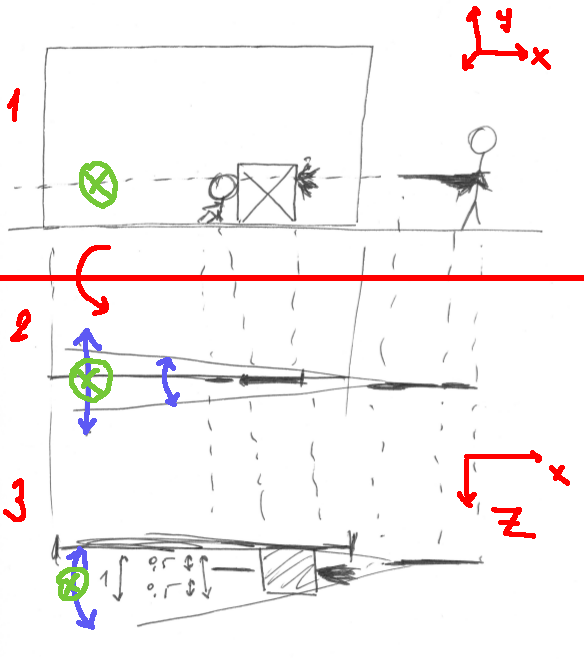
\includegraphics[height=0.59\textheight]{img/eps/up2.eps}
	\caption{Вид сбоку - 1, вид сверху - 2 и 3 \\ Настоящий вид сверху - 2,  С виртуальным объемом - 3\\ Зеленый цвет - прицел, Сиреневый - разброс.}
	\label{img:layers}
\end{figure}



\subsection{Ближний бой}
\subsubsection{<<Ячейки боя>>}
Ближний бой в игре очень рисковое дело потому что никогда не знаешь чем это может кончиться для тебя. Основная идея ближнего боя состоит в том, что у игрока как и у его противника есть определенное количество так называемых \textit{<<Ячеек боя>>}, как правило их 4 или 5 штук. У гг их 4, у большинства противников 5, а у некоторых их может быть даже 10 - понятно что даже не зная как это работает, с таким противником в ближний бой лучше не вступать. 

\subsubsection{Захваты}
Стоит начать с того что не каждый ближний бой превращается в пошаговый поединок. В игре у всех в том числе и у игрока есть возможность нормального боя с холодным оружием в руках. Так же у всех в игре есть возможность сражаясь в ближнем бою время от времени буквально втягивать противника в поединок с ячейками. Делается это с помощью специальных умений, хотя де-факто работает как специальные захваты в файтингах. Те кто хоть немного играл в свое время в файтинги знает что от захватов противника можно увернуться - так же и тут. Захваты имеют свое время перезарядки - если захват не удался, то время перезарядки в таком случае уменьшается в двое. Так или иначе спамить захватами не получится, потому что это не пошаговая аркада.

\subsubsection{Поединок}
Если все же увернуться не удалось или не захотелось. то поединок в ближнем бою каждый раз развивается по одинаковому сценарию - у игрока на экране всплывает \textit{<<N>>} пустых слотов равное количеству активных ячеек боя. Затем игроку следует эти ячейки заполнить \textit{<<Фишками атаки>>} или \textit{<<Фишками защиты>>}. Каждая фишка атаки предполагает одну собственно атаку тем чем выбрал игрок - это может быть даже пистолет в ближнем бою, в свою очередь \textit{Фишки защиты} направлены на то, что бы эти атаки отражать, но только те что были угаданы - иначе говоря фишка защиты от атаки пистолетом действует только против пистолета, если же этот пистолет использован не был, то фишка просто не используется.

\subsubsection{Избиение}
После каждого боя - неважно закончился он удачно или нет, одна ячейка боя уходит на перезарядку на 30 секунд (это значение будет балансироваться). Если ячеек больше не остается, то игрок или противник, в зависимости кто все ячейки потерял, просто получает все удары без исключений. Иначе говоря без активных ячеек боя - ближний бой превращается в избиение. Сделано было это в первую очередь что бы динамизм драк не проседал когда дело доходит до частых рукопашных, ведь в таком случае целый бой де-факто стал пошаговым, особенно так бы происходило в случаях когда персонажа окружают и начинают драться с ним в рукопашную - очевидно что нет смысла в такой ситуации тянуть время и потому когда все ячейки сгорают, а в данной ситуации это происходит очень быстро, то драка заканчивается тем чем заканчивается каждый неравный бой 1 против всех.


\subsubsection{Противники заточенные под ближний бой}
В игре периодически появляются такие противники, у которых вся механика построена на ближнем бою, причем не обыкновенном ближнем бою как это встречается у слабых <<NPC>>, а именно на поединках. У таких противников как может быть по 10 и более ячеек боя, очень высокая скорость передвижения и очень маленькое время перезарядки захвата. Все это означает, что с таким противником в бой на условиях врага лучше не вступать вообще. Однако даже у таких монстров есть свои слабые места - все враги зачастую используют одну любимую тактику и если ее разгадать, то даже очень сильный враг становится беззащитным. 


\section{Поле зрения ИИ}
Все <<NPC>> за исключением толпы, которую по правде говря сложно причислять к <<NPC>>, обладают зрением базирующимя на приеме рейтрейсинга\footnote{\emph{http://www.redblobgames.com/articles/visibility/}}, тут кажется нечего объяснять - все и так понятно из рисунка.\\
\begin{wrapfigure*}{l}{\linewidth}
	\centering
	\begin{center}
		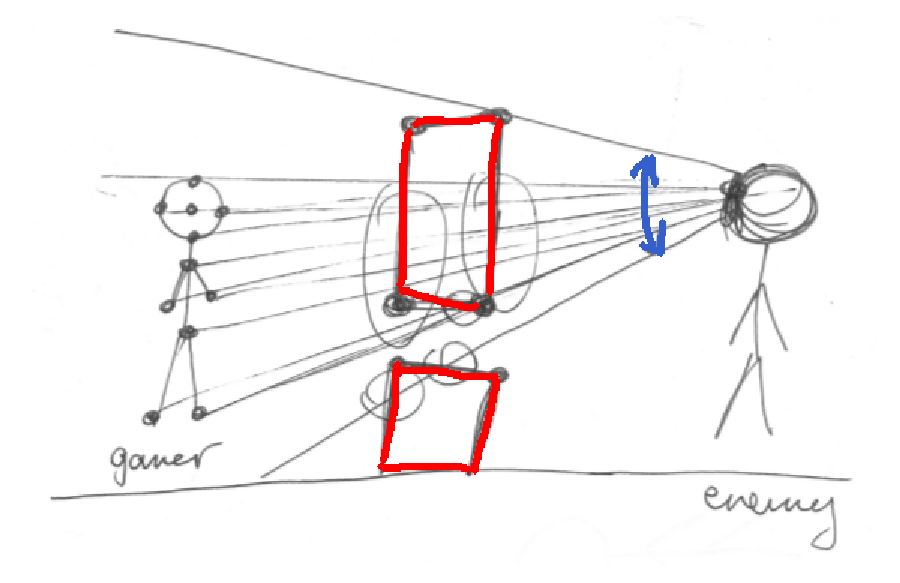
\includegraphics[width=\linewidth]{img/eps/rc1.eps}
	\end{center}
\end{wrapfigure*}



\newpage
\chapter[Повествование с технической стороны]{Повествование с технической\\ стороны}
Эта глава должна пролить чуть больше света на не очень хитрые манипуляции с движком игры\footnote{\emph{https://goo.gl/xijPjJ}}, делающие процесс повествования более оригинальным, в целом более кинематографическим. Как и остальные главы - эта тоже будет дополняться контентом в процессе разработки и появления новых идей касательно формы повествования.
\newpage

\section{Огранивение FPS}
В игре количество отображаемых кадров в секунду искусственно ограничено до 24 + 1.
В первую очередь это мотивировано восприятием - во время динамичных сцен 24 FPS заставляют наблюдателя фокусироваться на главном происходящем уводя все остальное на задний план. Дополнительный кадр нужен для страховки от проседания FPS, которое часто возникает на верхней границе лимита независимо от видеокарты.\\

\section{Манимпуляции с камерой}
\subsection{Каширование}
Каширование или искусственное наложение черных рамок в определенные моменты событий не являются чем то новым в кино, однако в играх такой прием еще не использовался, если автору не изменяет память. Данный примем можно расценивать как одну из попыток создать новый способ повествования в играх. Хорошим примером использование данной техники в кино могут послужить фильмы Нолана - например Интерстеллар. Технически это решение можно отнести в категорию пост-обработки.

\subsection{Композиция кадра}
Положение и поведение камеры очень важно не только в кино, но и в играх, особенно в двухмерных. Хорошо поставленный кадр способен задать настрой повествования и вычленять из него самое важное. Камера в игре в зависимости от контекста может быть жестко привязанной к персонажу или наоборот плавать с опозданием или опереженением - располагая персонажа в нужной части экрана.\footnote{\emph{https://habrahabr.ru/post/272933/}}\\


\section{Пост-обработка}
Сначала идет основной рендер, потом дополнительный. Делать с полученной из первоначального рендерирования картинкой можно что угодно - самый простой пример снизить или добавить контрастность, однако не стоит недооценивать даже такие маленькие изменения, ведь даже небольшое изменение контраста способно повлиять на тон повествования.


\part{Заключение}

\end{document}
